% ============================================================
% IV. CAPSULE APPROXIMATION METHOD
% ============================================================
\section{Capsule Approximation Method}
\label{sec:method}

This section describes the core capsule-fitting pipeline, which converts a single link mesh into a set of covering capsules.
The pipeline is executed independently for each link that contains mesh geometry, operating in the link's coordinate frame after applying the mesh-origin transform.

% ---- A. Problem Formulation ----
\subsection{Problem Formulation}

Let $\mathcal{M} = (V, F)$ be a triangular mesh for a single robot link, where $V = \{\mathbf{v}_i \in \mathbb{R}^3\}_{i=1}^{n}$ are the vertex positions and $F$ is the face index set.
A capsule $c$ is parameterized by its segment endpoints $\mathbf{p}_0, \mathbf{p}_1 \in \mathbb{R}^3$ and radius $r > 0$:
\begin{equation}
c = \{ \mathbf{x} \in \mathbb{R}^3 \mid d(\mathbf{x}, \overline{\mathbf{p}_0\mathbf{p}_1}) \leq r \},
\end{equation}
where $d(\mathbf{x}, \overline{\mathbf{p}_0\mathbf{p}_1})$ is the Euclidean distance from $\mathbf{x}$ to the line segment $\overline{\mathbf{p}_0\mathbf{p}_1}$.

The goal is to find a set of capsules $\mathcal{C} = \{c_1, \dots, c_k\}$ satisfying:
\begin{align}
&\text{Coverage:} \quad \forall \mathbf{v} \in V,\; \min_{c \in \mathcal{C}} d(\mathbf{v}, c) \leq 0, \label{eq:coverage}\\
&\text{Compactness:} \quad k \leq K_{\max}, \label{eq:budget}\\
&\text{Tightness:} \quad \text{minimize excess volume and radius inflation.} \label{eq:tightness}
\end{align}

Coverage (\Cref{eq:coverage}) requires every mesh vertex to lie inside at least one capsule.
The primitive budget (\Cref{eq:budget}) limits the total number of capsules per link.
Tightness (\Cref{eq:tightness}) is measured through a combination of capsule union volume relative to the link's axis-aligned bounding box (AABB) volume and a radius-inflation profile along each capsule's axis.

Figure~\ref{fig:method_schematic} illustrates the full pipeline visually on a representative link: PCA axis computation, cross-section slicing, circle fitting, and the resulting capsule chain.

\begin{figure}[t]
\centering
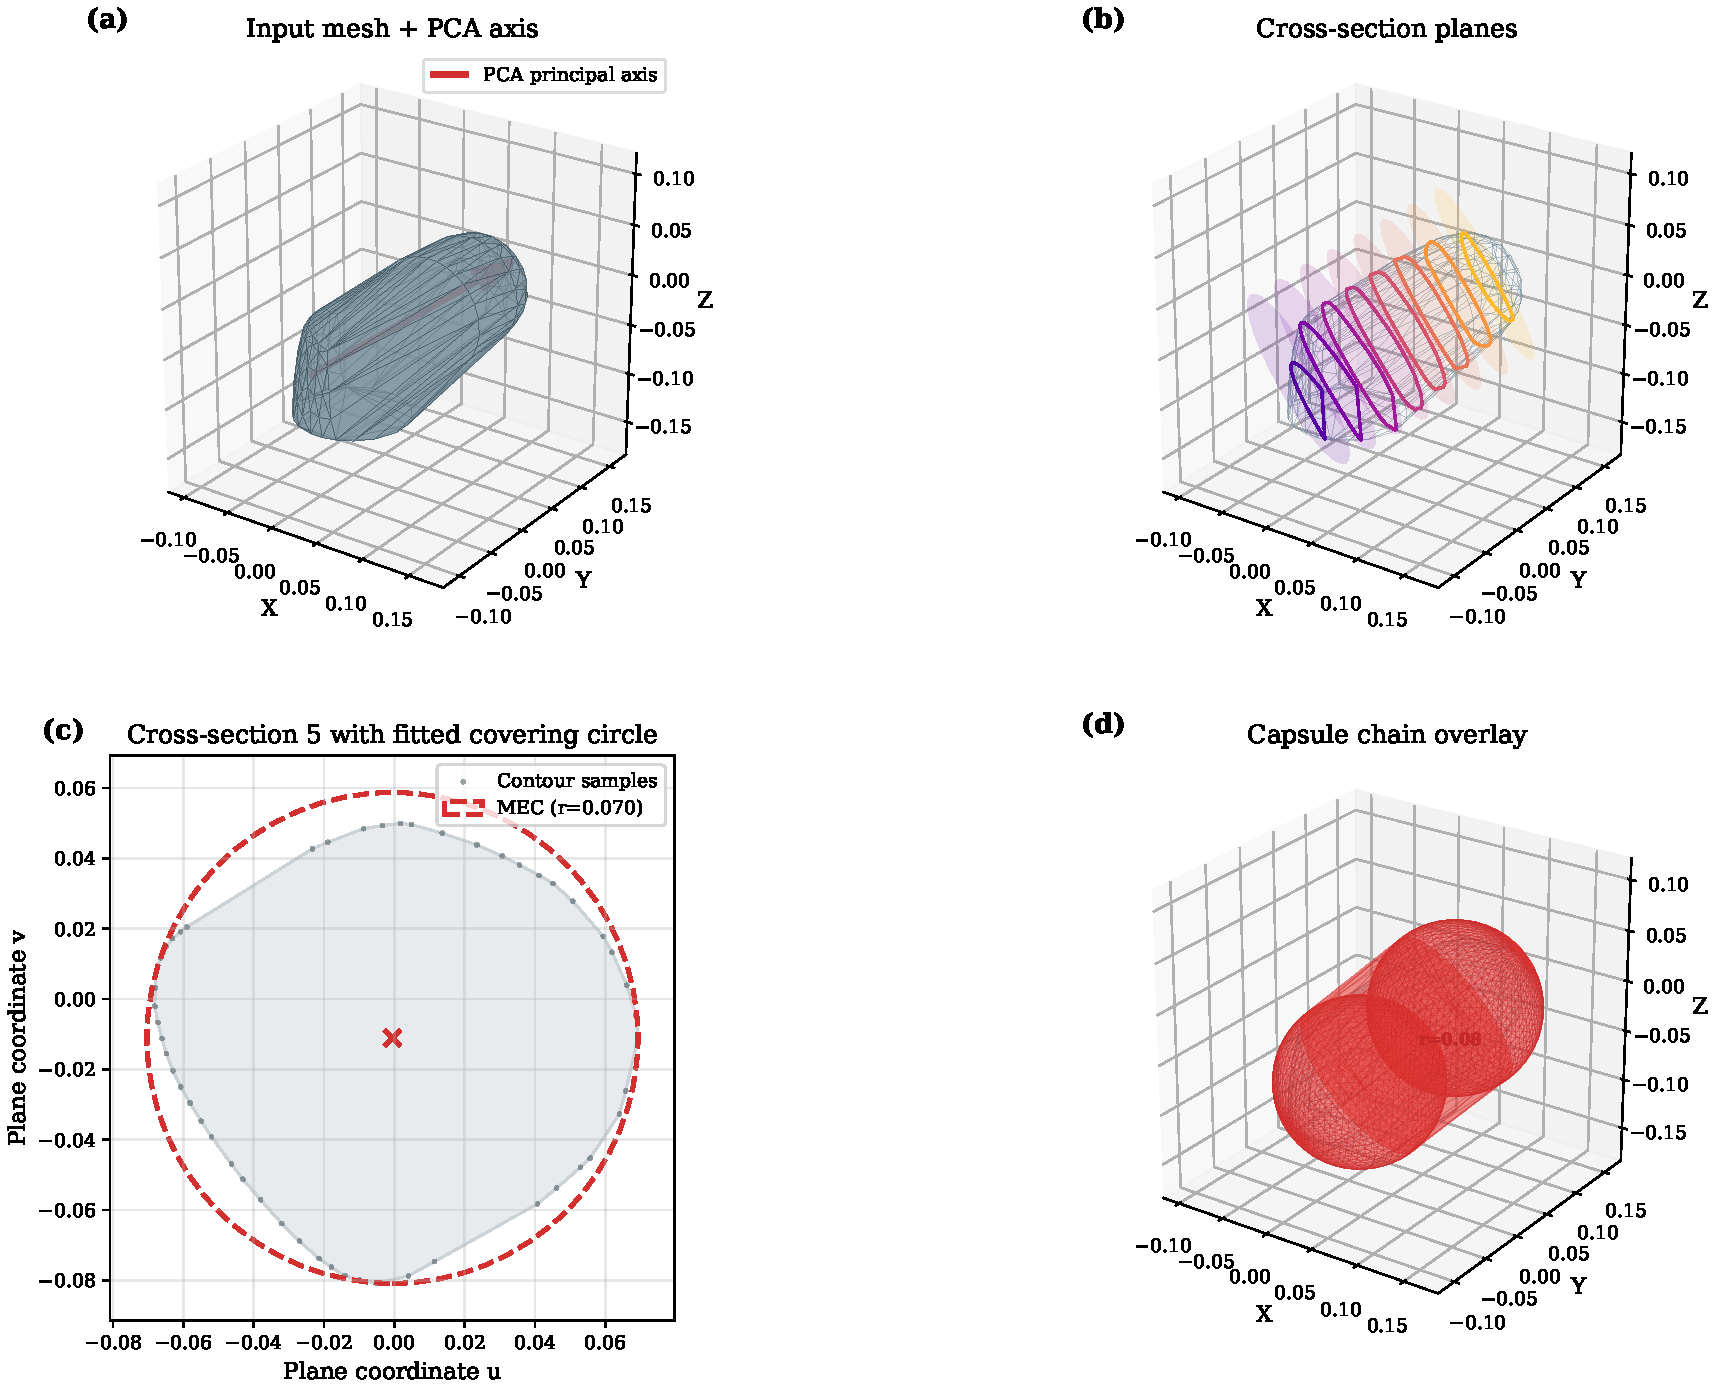
\includegraphics[width=\linewidth]{figures/capsule_method_schematic.pdf}
\caption{Overview of the capsule fitting pipeline on a representative FR3 link (link3). (a) Input mesh with PCA principal axis overlaid. (b) Cross-section planes perpendicular to the principal axis with extracted contours. (c) 2D cross-section contour with its minimum enclosing circle (MEC). (d) Resulting capsule chain overlaid on the original mesh.}
\label{fig:method_schematic}
\end{figure}

% ---- B. Mesh Preparation ----
\subsection{Mesh Preparation and Frame Handling}

Before fitting, the pipeline resolves the mesh source from the URDF.
For the default visual-mesh source, any non-OBJ/STL visual meshes (e.g., COLLADA format files) are converted to OBJ format in a Python preprocessing step using Trimesh~\cite{trimesh}.
The loaded mesh is then processed through ManifoldPlus~\cite{huang2022manifoldplus} to obtain a watertight manifold, which is required for robust cross-section slicing.
The watertight mesh vertices are transformed from the mesh-local frame to the link frame using the origin transform specified in the URDF element (translation $\mathbf{T}$ and rotation matrix $R$):
\begin{equation}
\mathbf{v}^{\mathrm{lf}} = \mathbf{T} + R\,\mathbf{v}^{\mathrm{mesh}}.
\end{equation}

After fitting, the capsules are grown against the \emph{original} (non-manifold) mesh vertices in the link frame to guarantee coverage of the real collision surface, which may differ from the watertight approximation.

% ---- C. Principal-Axis Sectioning ----
\subsection{Principal-Axis Sectioning}

The pipeline computes the principal axis of the link mesh via principal component analysis (PCA).
Let $\bar{\mathbf{v}}$ be the mesh centroid. The covariance matrix is
\begin{equation}
\Sigma = \frac{1}{n} \sum_{i=1}^{n} (\mathbf{v}_i - \bar{\mathbf{v}})(\mathbf{v}_i - \bar{\mathbf{v}})^{\mathsf{T}}.
\end{equation}
The eigenvector corresponding to the largest eigenvalue defines the principal axis $\mathbf{u}$, which serves as the ``bone direction'' for sectioning.

The mesh is sliced with $N$ planes perpendicular to $\mathbf{u}$ at uniformly spaced positions $t_k$ along the axis, using the midpoint spacing $t_k = t_{\min} + (k + 0.5)(t_{\max} - t_{\min}) / N$ (centered in each interval to avoid degenerate cuts at planar end caps).
For each slice, triangle-plane intersections are computed: each triangle that straddles the plane contributes a 2D line segment in the plane's local basis $(\mathbf{e}_1, \mathbf{e}_2)$.
These segments are chained into closed polygonal contours by iteratively matching segment endpoints, producing a set of 2D cross-section contours $\{P_j\}$ per plane.

The section count $N$ is a user-configurable parameter; typical values range from 2 (coarse) to 8 (fine).

% ---- D. Cross-Section Circle Fitting ----
\subsection{Cross-Section Circle Fitting}

Each cross-section contour $P$ is approximated by a set of covering circles in the 2D plane.
A circle is represented as $( \mathbf{o}, r )$ with center $\mathbf{o} \in \mathbb{R}^2$ and radius $r > 0$.
The coverage condition is that every sampled point of the contour lies within at least one circle.

\paragraph{Minimum enclosing circle (MEC).}
For a single circle, the minimum enclosing circle is computed via Welzl's randomized algorithm~\cite{welzl1991mec} with a fixed random seed for determinism.
A circle is considered to cover the contour when its circle-outside-area (COA)~\cite{wu2018capsule}---the area of the circle lying outside the contour polygon---falls below a threshold $\tau$.

\paragraph{Adaptive multi-circle fitting.}
When adaptive circle fitting is enabled, the pipeline starts with one MEC and iteratively refines it using Lloyd-style clustering.
At each step, the circle with the largest COA is split into two via k-means ($k = 2$) on its assigned contour samples.
Each resulting cluster is replaced with a fresh MEC, and the process repeats until the total COA falls below $\tau$ or the maximum circle count per section is reached.
The COA for a circle $(\mathbf{o}, r)$ relative to a polygon $P$ is computed as the signed sum of circular-segment areas between the circle and each polygon edge, following Wu et al.~\cite{wu2018capsule}:
\begin{equation}
\mathrm{COA}(\mathbf{o}, r, P) = \begin{cases}
A_{\mathrm{in}}, & \mathbf{o} \text{ inside } P, \\
\pi r^2 + A_{\mathrm{in}}, & \mathbf{o} \text{ outside } P,
\end{cases}
\label{eq:coa}
\end{equation}
where $A_{\mathrm{in}}$ is the signed accumulated area of circular segments inside the polygon.

\paragraph{Fixed-count circle fitting.}
When adaptive fitting is disabled (the default), a fixed number of circles $M$ (the per-section maximum) is fitted per section using deterministic farthest-point initialization followed by $k$-means clustering.

% ---- E. Capsule Construction Across Sections ----
\subsection{Capsule Construction Across Sections}

The 2D circles from adjacent section planes are linked into 3D capsules through a matching process.

Let $\{c_{i}^{(p)}\}$ be the set of circles fitted to section plane $p$ at position $t_p$.
Each 2D circle center is mapped to 3D:
\begin{equation}
\mathbf{o}_{i}^{(p)} = \bar{\mathbf{v}} + t_p \mathbf{u} + o_x^{(p)} \mathbf{e}_1 + o_y^{(p)} \mathbf{e}_2,
\end{equation}
where $(o_x, o_y)$ are the 2D circle center coordinates in the section plane basis.

Starting from the first section, each circle maintains an active chain.
At each subsequent section, each active circle is matched to the nearest unused circle in the new section by Euclidean distance in the 2D plane (equivalent to nearest-center matching after subtracting axial offset).
A capsule is emitted between the matched pairs with radius $r = \max(r_{\text{prev}}, r_{\text{next}})$:
\begin{equation}
c = \{ \mathbf{p}_0 = \mathbf{o}_{\text{prev}}, \mathbf{p}_1 = \mathbf{o}_{\text{next}}, r = \max(r_{\text{prev}}, r_{\text{next}}) \}.
\end{equation}
Unmatched circles in the new section start new chains.
Chains that fail to match terminate.

After all sections are processed, endpoint sections are extended to the mesh axial extrema $\mathbf{v} \cdot \mathbf{u}$ to ensure coverage at the link extremities.

% ---- F. Coverage-Preserving Refinement ----
\subsection{Coverage-Preserving Refinement}

The initial capsules undergo a series of refinement passes that jointly improve tightness while preserving coverage.

\paragraph{Collinear merging.}
Adjacent capsules that are approximately collinear (axial dot product $> 0.3$) and have similar radii (difference $< 15\%$) are merged into a single capsule spanning the full extent.
This reduces the capsule count without affecting coverage.

\paragraph{Radius growth (grow to cover).}
Every mesh vertex is assigned to its nearest capsule by point-to-segment distance.
Each capsule's radius is then expanded to at least the maximum distance of its assigned vertices, ensuring \Cref{eq:coverage} holds.

\paragraph{Endpoint span shrinkage.}
Each capsule's axis endpoints $(\mathbf{p}_0, \mathbf{p}_1)$ are optimized by searching over candidate shrink amounts while re-computing the required coverage radius.
The candidate that minimizes capsule volume while maintaining coverage is selected.
This process is iterated until convergence.

\paragraph{Inflation-based splitting.}
When a capsule exhibits excessive radius inflation---measured by the ratio $r / r_{\text{median\_bin}}$, where $r_{\text{median\_bin}}$ is the median of per-bin maximum vertex distances along the capsule axis---the pipeline attempts to split the capsule at the bin where inflation is worst.
Each split produces two child capsules whose radii are re-grown from the assigned vertex subsets.
A split is accepted only if it reduces the capsule union volume or improves the radius-inflation metric above a threshold $\delta_{\min}$.
Splitting is also triggered when the capsule union volume relative to the link AABB volume exceeds a configured ceiling $\eta_{\max}$.

\paragraph{Nested-capsule pruning.}
After refinement, capsules that are entirely contained within another capsule are removed.
A capsule $c_i$ is nested in $c_j$ when both of $c_i$'s end-spheres (points $\mathbf{p}_0^i$ and $\mathbf{p}_1^i$, each inflated by $r_i$) lie within $c_j$, i.e.:
\begin{equation}
d(\mathbf{p}_0^i, \overline{\mathbf{p}_0^j\mathbf{p}_1^j}) + r_i \leq r_j \quad\text{and}\quad
d(\mathbf{p}_1^i, \overline{\mathbf{p}_0^j\mathbf{p}_1^j}) + r_i \leq r_j.
\end{equation}
Since capsules are convex, this guarantees $c_i \subseteq c_j$, so removing $c_i$ does not affect coverage.

\paragraph{Budget enforcement.}
If after refinement the capsule count exceeds the per-link budget $K_{\max}$, the pipeline iteratively removes the capsule whose removal minimizes the resulting capsule union volume, re-growing the remaining capsules to maintain coverage after each removal.

% ---- G. URDF-Compatible Emission ----
\subsection{URDF-Compatible Emission}

URDF does not provide a native capsule geometric element.
Each capsule is therefore decomposed into one cylinder and two spheres for URDF output:
\begin{itemize}
    \item A \texttt{<cylinder>} with radius $r$ and length $\|\mathbf{p}_1 - \mathbf{p}_0\|$, positioned at the capsule midpoint $\frac{1}{2}(\mathbf{p}_0 + \mathbf{p}_1)$ and oriented such that the cylinder axis aligns with $\mathbf{p}_1 - \mathbf{p}_0$ (via a quaternion rotation from the default $z$-axis).
    \item Two \texttt{<sphere>} elements with radius $r$, one at each endpoint $\mathbf{p}_0$ and $\mathbf{p}_1$.
\end{itemize}
A degenerate capsule with $\|\mathbf{p}_1 - \mathbf{p}_0\| \approx 0$ is emitted as a single \texttt{<sphere>}.

Simultaneously, the canonical capsule parameters $(\mathbf{p}_0, \mathbf{p}_1, r)$ are written to the JSON sidecar.
This dual output ensures that the URDF is immediately usable in any URDF-compatible simulator while preserving the analytic capsule representation for downstream code that supports capsule collision directly.
